\documentclass{article}
\usepackage[final]{nips_2017}
\usepackage[utf8]{inputenc} % allow utf-8 input
\usepackage[T1]{fontenc}    % use 8-bit T1 fonts
\usepackage{hyperref}       % hyperlinks
\usepackage{url}            % simple URL typesetting
\usepackage{booktabs}       % professional-quality tables
\usepackage{amsfonts}       % blackboard math symbols
\usepackage{nicefrac}       % compact symbols for 1/2, etc.
\usepackage{microtype}      % microtypography
\usepackage{graphicx}
\usepackage{wrapfig}
\title{Family kinship Recognition Using Deep Learning}

\author{
  Bruce Jianye Liu\\
  Department of Computer Science\\
  Stanford University\\
  \texttt{bruceliu@stanford.edu} \\
}


\begin{document}
% \nipsfinalcopy is no longer used

\begin{center}

\includegraphics[width=3cm, height=0.7cm]{CS230}
\end{center}

\maketitle

\section{Problem Description}
Half of genetic information is passed down from parents to children. Therefore
people biologically related share delicate similiarities. This declicacy could
be caught by human eyes, by looking at family photos. While computer vision
performance improving in the decade, it becomes impossible to use deep learning
model to capture the different. Kinship recognition could lead variety of
usefull applications in reality such as missing-children and parents matching,
family album organization, socal networking apps, lost sibling/relatives
searching, crime investigation. In this paper, we propose a fine-tuned FaceNet
model to identify the relationship between two faces -- parent-children, sibling-sibling, or none-kinship.

\section{Related Works}

It might be hard to achieve higher accuracy since people without any family
kinship would look simliar to each other. There are other metrics that we could
consider to determine if the kinship exists. Such information includes hands
shape, nail types, foot toes, ears, hairs. Due to time limitation and team
size, we aren't able to collect this data. Otherwise the prediction would
improve a lot.

Kin recognition work mainly focus on kinship verification, to decide whether
two faces have kinship, family classification, classifing a face to a family,
and family member regcontion, determining 2 faces siblings or parents. Over the
past decades, many methods has been proposed on this research, including
hand-crafted feature, face ecnodings, and metric learning[3].

\section{Dataset}

\begin{wrapfigure}{l}{0.25\textwidth}
\caption{108x124 face sample}
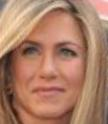
\includegraphics{img/P00241_face0}
\end{wrapfigure}

We are going to use Families In The Wild (FIW) Database[1]. FIW is the largest
and most comprehensive database available for kinship recognition. We use
version 0.1.2 at writing time, which include 13,188 faces from 1018 families.
Event though it has 11 kinship types, father-daughter (F-D), father-son (F-S),
mother-daughter (M-D), mother-son (M-S), brother-brother (B-B), sister-sister
(S-S), grandfather-granddaughter (GF-GD), grandfather-grandson (GF-GS),
grandmother-granddaughter (GM-GD), grandmother-grandson (GM-GS), to our study,
siblings and parent-child types are what we are going to use. Adding up 64669
F-D, 46143 F-S, 68935 M-D, 48940 M-S types, we get 22687 parent-child photos
while sibling types contains 55937 photos. All face images are 108*124*3 size.
The same face data is generated by selecting pictures with the same FaceID.
Non-related picture pairs are generated with pictures in the Family folder and
one of the faces in the family.

\begin{table}[h]
	\centering
	\begin{tabular}{ | c || r r | }
		\hline
		\multicolumn{3}{|c|}{face-pair image distribution} \\
		\hline
		pair types&face-pair number&percentage\\
		\hline
			parent-child & 228,687 &21.17\% \\
			siblings & 55,937 & 5.18\% \\
			same & 230,938 & 21.38\% \\
			unrelated & 564,496 & 52.27\% \\
		\hline
			& 1,080,058 & \\
		\hline
	\end{tabular}
	\caption{Training data distribution}
	\label{table:1}
\end{table}

Table 1 distrubtion may affect our model less confident to predict sibling
faces, while we may could do well on P-C, same faces, and non-related images.

There are another smaller family dataset KinFaceW-I and KinFaceW-II, which
includes 533 pairs of parent-child type images.

We divided 95 of the images as training set, 5 percent as test set.

\section{Methods and Models}

Since FIW includes pretrained embedding data of each faces, every face image is
encoded in 512D embedding using VGG-Face net. With this data, I built a deep
neural classifier with a softmax layer of 4 labels. I stacked 2 embedding
vectors into 1024D as the input data, passed them 4 layers network which
contain 512, 128, 64, 4 hidden units, separately. The first 3 layers is RELU
activation, and the final one is softmax.The model is initialised with "He" and
is trained with learning rate 0.05.

The result is not ideal. I am not able to train it very well with my laptop
although I managed make the model work. I can't make through the first training
epoch. Loading the whole data into memory is still quite expensive on my local
machine, taking nearly 30 seconds. Going through 200 iterations costs about 20
minutes. After talking with TAs, he suggested to use aws gpu instance. It seems
this model I coded from scratch with numpy couldn't take advantage of GPU
processing power. The next milestone model could be any machine learning
framework such as Keras, Tensorflow or pytorch.

FaceNet[2] performs very well in face recognition tasks. I am going to tweak the
model little bits to create new model to classify image pairs.

\begin{figure}[h]
	\caption{Our modified model}
	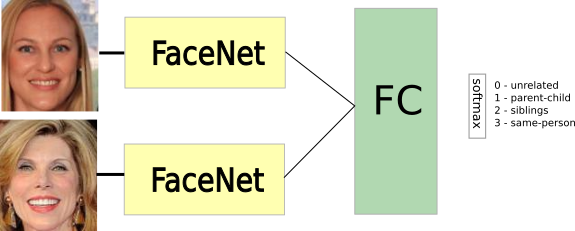
\includegraphics[width=1\textwidth]{img/model_pic}
\end{figure}

One of the facenet implementation models is ResNet v1, which possibly have a
better performance than VGG-Face net. However it is very expensive to train as
it contains over 1 million parameters. Face kinship and face recogintion are
very similar problems. I am going to take pretrained model, fitting it my new
model, retain them. This could speed up the trainning process.

github repository: https://github.com/brucelau-github/cs230

\newpage
\section*{References}
\medskip
\small
[1] Robinson, Joseph P., et al. Families in the Wild (FIW): Large-Scale Kinship
Image Database and Benchmarks. {\it Proceedings of the 2016 ACM on Multimedia
Conference} - MM '16, 2016, doi:10.1145/2964284.2967219.

[2] Schroff, F., Kalenichenko, D., \& Philbin, J. (2015). FaceNet: A unified
embedding for face recognition and clustering. {\it 2015 IEEE Conference on
Computer Vision and Pattern Recognition (CVPR)}. doi: 10.1109/cvpr.2015.7298682

[3] Wang, S., Robinson, J. P., \& Fu, Y. (2017, May). Kinship verification on
families in the wild with marginalized denoising metric learning. {\it In 2017 12th
IEEE International Conference on Automatic Face \& Gesture Recognition (FG 2017)
(pp. 216-221). IEEE}.

[4] Szegedy, C., Ioffe, S., Vanhoucke, V., \& Alemi, A. A. (2017, February).
Inception-v4, inception-resnet and the impact of residual connections on
learning. In {\it Thirty-first AAAI conference on artificial intelligence}.

\end{document}
